%%%%%%%%%%%%%%%%%%%%%%%%%%%%%%%%%%%%%%%%%
% Beamer Presentation
% LaTeX Template
% Version 1.0 (10/11/12)
%
% This template has been downloaded from:
% http://www.LaTeXTemplates.com
%
% License:
% CC BY-NC-SA 3.0 (http://creativecommons.org/licenses/by-nc-sa/3.0/)
%
%%%%%%%%%%%%%%%%%%%%%%%%%%%%%%%%%%%%%%%%%

%----------------------------------------------------------------------------------------
%	PACKAGES AND THEMES
%----------------------------------------------------------------------------------------

\documentclass{beamer}

\mode<presentation> {

% The Beamer class comes with a number of default slide themes
% which change the colors and layouts of slides. Below this is a list
% of all the themes, uncomment each in turn to see what they look like.

%\usetheme{default}
%\usetheme{AnnArbor}
%\usetheme{Antibes}
%\usetheme{Bergen}
%\usetheme{Berkeley}
%\usetheme{Berlin}
%\usetheme{Boadilla}
%\usetheme{CambridgeUS}
%\usetheme{Copenhagen}
%\usetheme{Darmstadt}
%\usetheme{Dresden}
%\usetheme{Frankfurt}
%\usetheme{Goettingen}
%\usetheme{Hannover}
%\usetheme{Ilmenau}
%\usetheme{JuanLesPins}
%\usetheme{Luebeck}
\usetheme{Madrid}
%\usetheme{Malmoe}
%\usetheme{Marburg}
%\usetheme{Montpellier}
%\usetheme{PaloAlto}
%\usetheme{Pittsburgh}
%\usetheme{Rochester}
%\usetheme{Singapore}
%\usetheme{Szeged}
%\usetheme{Warsaw}

% As well as themes, the Beamer class has a number of color themes
% for any slide theme. Uncomment each of these in turn to see how it
% changes the colors of your current slide theme.

%\usecolortheme{albatross}
%\usecolortheme{beaver}
%\usecolortheme{beetle}
%\usecolortheme{crane}
%\usecolortheme{dolphin}
%\usecolortheme{dove}
%\usecolortheme{fly}
%\usecolortheme{lily}
%\usecolortheme{orchid}
%\usecolortheme{rose}
%\usecolortheme{seagull}
%\usecolortheme{seahorse}
%\usecolortheme{whale}
%\usecolortheme{wolverine}

%\setbeamertemplate{footline} % To remove the footer line in all slides uncomment this line
%\setbeamertemplate{footline}[page number] % To replace the footer line in all slides with a simple slide count uncomment this line

%\setbeamertemplate{navigation symbols}{} % To remove the navigation symbols from the bottom of all slides uncomment this line
}

\usepackage{graphicx} % Allows including images
\graphicspath{ {Figures/} }
\usepackage{booktabs} % Allows the use of \toprule, \midrule and \bottomrule in tables
\usepackage{mathtools}
\usepackage[mathscr]{euscript}
\usepackage{amssymb}
\usepackage{amsmath}

\AtBeginSection[]
{
  \begin{frame}<beamer>
    \frametitle{Outline}
    \tableofcontents[currentsection]
  \end{frame}
}
%----------------------------------------------------------------------------------------
%	TITLE PAGE
%----------------------------------------------------------------------------------------

\title[Reinforcement Learning]{Reinforcement Learning} % The short title appears at the bottom of every slide, the full title is only on the title page

\author{Jack Lanchantin} % Your name
%\institute[UCLA] % Your institution as it will appear on the bottom of every slide, may be shorthand to save space
%{
%University of California \\ % Your institution for the title page
%\medskip
%\textit{john@smith.com} % Your email address
%}
\date{\today} % Date, can be changed to a custom date

\begin{document}

\begin{frame}
\titlepage % Print the title page as the first slide
\end{frame}

\begin{frame}
\frametitle{Outline} % Table of contents slide, comment this block out to remove it
\tableofcontents % Throughout your presentation, if you choose to use \section{} and \subsection{} commands, these will automatically be printed on this slide as an overview of your presentation
\end{frame}

%----------------------------------------------------------------------------------------
%	PRESENTATION SLIDES
%----------------------------------------------------------------------------------------
%------------------------------------------------
\section{Reinforcement Learning} % Sections can be created in order to organize your presentation into discrete blocks, all sections and subsections are automatically printed in the table of contents as an overview of the talk

\begin{frame}
\frametitle{Reinforcement Learning}
\begin{itemize}
\item \textbf{Framing of the problem of learning from interaction to achieve a goal.}
\item \textbf{Agent}: learner and decision maker
\item \textbf{Environment}: what the learner interacts with (everything outside the agent)
\item Agent selects actions and the environment responds to those actions and presents new situations
\end{itemize}
\end{frame}

%------------------------------------------------

\begin{frame}
\frametitle{Reinforcement Learning}

\begin{figure}[t]
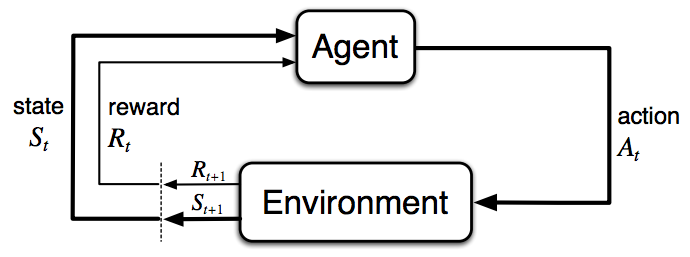
\includegraphics[scale=0.3]{AgentEnvironment}
\centering
\end{figure}

\begin{itemize}
\item At each time step $t$, the agent receives the environment \textbf{state} $S_t$ $\in$ $\mathscr{S}$, 
 and the agent then selects an \textbf{action} $A_t \in$ $\mathscr{A}$($S_t$) 
   \begin{itemize}
   	\item $\mathscr{S}$ is the set of possible states (whatever information is available to the agent).
        \item $\mathscr{A}$($S_t$) is set of actions available in state $S_t$
      \end{itemize}
\item One time step later, the agent receives a \textbf{reward}, $R_{t+1} \in$ $\mathscr{R}$ $\subset$ $\mathbb{R}$,
and ends up in a new state $S_{t+1}$
\end{itemize}
\end{frame}

%------------------------------------------------

\begin{frame}
\frametitle{Reinforcement Learning}
\begin{columns}[c] % The "c" option specifies centered vertical alignment while the "t" option is used for top vertical alignment

\column{.45\textwidth} % Left column and width
At each step $t$,
\begin{itemize}
\item  The agent:
   \begin{itemize}
   	\item Receives state $S_t$
	\item Receives scalar reward $R_t$
	\item Executes action $A_t$
      \end{itemize}
\item The environment:
   \begin{itemize}
   	\item Receives action $A_t$
	\item Emits state $S_t$
	\item Emits scalar reward $R_t$
      \end{itemize}
\end{itemize}

\column{.5\textwidth} % Right column and width
\begin{figure}[t]
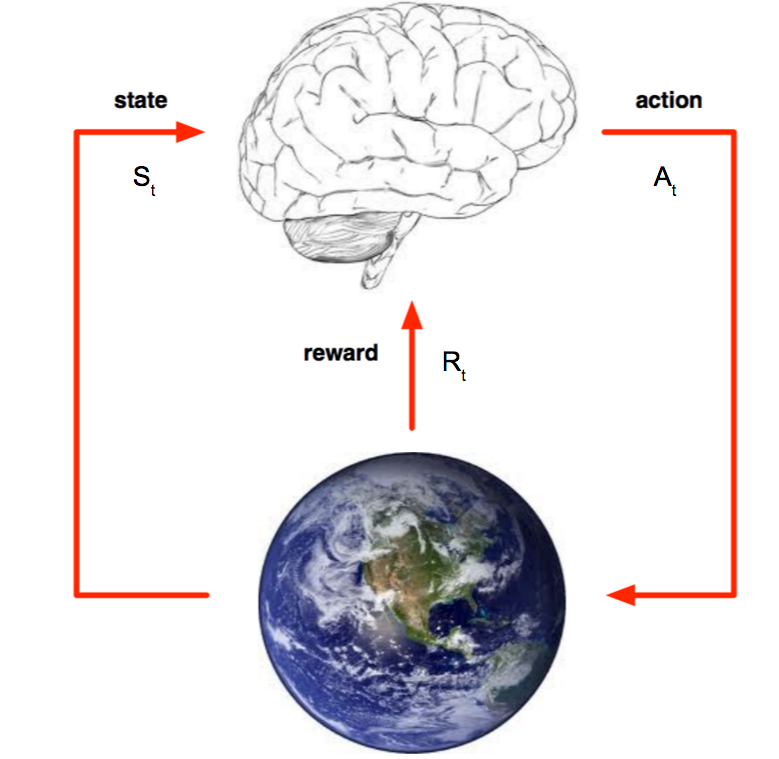
\includegraphics[scale=0.2]{EarthBrain}
\centering
\end{figure}

\end{columns}
\end{frame}


%------------------------------------------------

\begin{frame}
\frametitle{Reinforcement Learning Objective}
\begin{itemize}
\item If the sequence of rewards after time step $t$ is $R_{t+1}, R_{t+2}, R_{t+3},...$, then we want to maximize the return $G_t$
\item The agent chooses $A_t$ to maximize the discounted return: 
\begin{equation}
G_t = \sum_{k=0}^{T-t-1} \gamma^k R_{t+k+1}
\nonumber
\end{equation}
where $\gamma$ is the discount rate and 0 $\leq \gamma \leq$ 1. The closer $\gamma$ is to 1, the more the agent accounts for future rewards
\item \textbf{Select actions to maximise future reward}
\end{itemize}
\end{frame}

%------------------------------------------------
\section{Markov Decision Processes} % Sections can be created in order to organize your presentation into discrete blocks, all sections and subsections are automatically printed in the table of contents as an overview of the talk
%------------------------------------------------

%\subsection{Subsection Example} % A subsection can be created just before a set of slides with a common theme to further break down your presentation into chunks

\begin{frame}
\frametitle{Markov Property}
\begin{itemize}
\item Probability of transitioning to new state s' with reward r:
\small
\begin{equation}
p(s',r | s,a)=Pr\{S_{t+1}=s', R_{t+1}=r|S_0, A_0, R_1,...,S_{t-1},A_{t-1},R_t, S_t, A_t\}
\nonumber
\end{equation}
\normalsize
\item Probability with Markov assumption:
\begin{equation}
p(s',r | s,a) = Pr\{S_{t+1} = s', R_{t+1} = r | S_t = s, A_t = a\}
\nonumber
\end{equation}
\item Markov assumption allows us to predict the next state and expected rewards from knowledge of only the current state
   \begin{itemize}
   	\item Assume that the current state tells us everything we need to know for future (e.g. current state of checker board)
      \end{itemize}
\end{itemize}
\end{frame}

%------------------------------------------------



\begin{frame}
\frametitle{Markov Decision Processes}
\begin{itemize}
\item A reinforcement learning task that satisfies the Markov property is called a Markov Decision Process (MDP)
\item Given any state $s$ and action $a$, the probability of each possible pair of next state and reward ($s'$, $r$), is denoted
\begin{equation}
p(s',r | s,a) = Pr\{S_{t+1} = s', R_{t+1} = r | S_t = s, A_t = a\}
\nonumber
\end{equation}
\item From this probability representation, we can compute anything else we might need to know about the environment...
\end{itemize}
\end{frame}

%------------------------------------------------

\begin{frame}
\frametitle{Markov Decision Processes}
\begin{itemize}
\item State-transition probabilities:
\begin{equation}
p(s' | s,a) = Pr\{S_{t+1} = s' | S_t = s, A_t = a\} =  \sum_{r \in \mathscr{R} } p(s',r | s,a)
\nonumber
\end{equation}
\item Expected rewards for state--action pairs:
\begin{equation}
r(s,a) = \mathbb{E}[R_{t+1} | S_t = s, A_t = a] = \sum_{r \in \mathscr{R} } r \sum_{s' \in \mathscr{S} } p(s',r | s,a)
\nonumber
\end{equation}
\item Expected rewards for state--action--next-state triples:
\begin{equation}
r(s,a,s') = \mathbb{E}[R_{t+1} | S_t = s, A_t = a, S_{t+1}  = s'] =  \dfrac{ \sum_{r \in \mathscr{R} } r*p(s',r | s,a)}{p(s'| s,a)}
\nonumber
\end{equation}
\end{itemize}
\end{frame}

%------------------------------------------------

\begin{frame}
\frametitle{MDP Example}
\begin{itemize}
\item At each tilmestep $t$, a can-collecting robot decides whether it should (1) actively search for a can, 
(2) remain in place and wait for someone to bring it a can, or (3) go back to charging station to recharge its battery

\end{itemize}
\end{frame}


%------------------------------------------------
\section{Value Functions} % Sections can be created in order to organize your presentation into discrete blocks, all sections and subsections are automatically printed in the table of contents as an overview of the talk
%------------------------------------------------

%\subsection{Subsection Example} % A subsection can be created just before a set of slides with a common theme to further break down your presentation into chunks

%------------------------------------------------

\begin{frame}
\frametitle{Policies}
\begin{itemize}
\item At each time step, the agent implements a mapping $\pi$ from states to probabilities of selecting each possible action, where $\pi$ is called a \textbf{policy}
   \begin{itemize}
   	\item $\pi_t$($a|s$) = probability that $A_t$ = $a$ if $S_t$ = $s$
      \end{itemize}
\end{itemize}
\begin{block}{Reinforcement Learning Objective}
The agent's goal is to maximize the total amount of reward it receives over the long run by changing its policy as a result of its experience
\end{block}
\end{frame}

%------------------------------------------------

\begin{frame}
\frametitle{Value Functions}
\begin{itemize}
\item Almost all RL algorithms involve estimating value functions
\item \textbf{Value Functions:} functions of states (or state--action pairs) that estimate how good it is for the agent to be in a certain state (or to perform an action in a given state). 
   \begin{itemize}
   	\item "How good" is defined in terms of future rewards that can be expected (i.e. expected return)
      \end{itemize}
\end{itemize}
\end{frame}

%------------------------------------------------

\begin{frame}
\frametitle{State-Value Function for policy $\pi$}
\begin{itemize}
\item Recall that a policy $\pi$ maps a state $s$ and action $a$ to the probability $\pi(a|s)$ of doing $a$ when in $s$
\item The value of a state $s$ under policy $\pi$, denoted $v_\pi(s)$, is the \textbf{expected return when starting in state $s$ and following $\pi$ thereafter}:
\begin{equation}
v_\pi(s) = \mathbb{E}_\pi[G_t | S_t = s] = \mathbb{E}_\pi\Bigg[\sum_{k=0}^{\infty} \gamma^k R_{t+k+1} \Biggm\lvert S_t = s \Bigg]
\nonumber
\end{equation}
$\mathbb{E}_\pi[\cdot]$ is the expected value of a r.v. given the agent follows policy $\pi$
\end{itemize}
\end{frame}


%------------------------------------------------

\begin{frame}
\frametitle{Action-Value Function for policy $\pi$}
\begin{itemize}
\item The value of taking action $a$ in state $s$ under a policy $\pi$, denoted
$q_\pi(s,a)$, is the \textbf{expected return starting from s, taking the action a, and following policy $\pi$ thereafter}:
\begin{equation}
q_\pi(s) = \mathbb{E}_\pi[G_t | S_t = s, A_t = a] = \mathbb{E}_\pi\Bigg[\sum_{k=0}^{\infty} \gamma^k R_{t+k+1} \Biggm\lvert S_t = s, A_t = a \Bigg]
\nonumber
\end{equation}
\item Both $v_\pi$ and $q_\pi$ can be estimated from experience using Monte Carlo methods
\end{itemize}
\end{frame}


%------------------------------------------------

\begin{frame}
\frametitle{Computing Value Functions}
\begin{itemize}
\item Key idea of reinforcement learning is to use value functions to search for a good policy $\pi$
\item Can use dynamic programming techniques to compute optimal value functions, and thus find optimal policies 
\begin{align*}
v_\pi(s) &= \mathbb{E}_\pi[G_t | S_t = s] \\
&= \mathbb{E}_\pi\Bigg[\sum_{k=0}^{\infty} \gamma^k R_{t+k+1} \Biggm\lvert S_t = s \Bigg] \\
&= \sum_{a}\pi(a|s) \sum_{s',r} p(s',r|s,a) \big[ r + \gamma v_\pi(s') \big]
\nonumber
\end{align*}
\end{itemize}
\end{frame}

%------------------------------------------------

\begin{frame}
\frametitle{Optimal Value Functions}
\begin{itemize}
\item Solving a reinforcement learning task means finding a policy that achieves a
high reward over the long run
\item A policy $\pi$ is better than $\pi'$ if its expected return is $\geq$ to that of $\pi'$ for all states
   \begin{itemize}
   	\item I.e. $\pi \geq \pi'$ iff $v_\pi(s) \geq v_\pi'(s)$ for all $s \in \mathscr{S}$
      \end{itemize}
\end{itemize}
\end{frame}


%------------------------------------------------

\begin{frame}
\frametitle{Optimal Value Functions}
\begin{itemize}
\item The $optimal$ policies are denoted $\pi_{\ast}$
\item The \textit{optimal state-value functions} are denoted $v_{\ast}$ and defined:
\begin{equation}
v_{\ast}(s) = \underset{\pi}{\max} \ v_\pi(s) \ \textrm{for all} \ s \in \mathscr{S}
\nonumber
\end{equation}
\item The \textit{optimal action-value functions} are denoted $q_{\ast}$ and defined:
\begin{equation}
q_{\ast}(s,a) = \underset{\pi}{\max} \ q_\pi(s,a) \ \textrm{for all} \ s \in \mathscr{S} \textrm{ and } a \in \mathscr{A}
\nonumber
\end{equation}
\end{itemize}
\end{frame}

%------------------------------------------------

\begin{frame}
\frametitle{References}

Richard S. Sutton and Andrew G. Barto. Reinforcement Learning: An Introduction. MIT Press 2015.

\end{frame}

%------------------------------------------------

\end{document} 